\documentclass{article}

\def\ParSkip{} 
% Packages
\usepackage{amssymb,amsmath,amsthm,bbm}
\usepackage{verbatim,float,url,dsfont}
\usepackage{graphicx,subfigure,psfrag}
\usepackage{algorithm,algorithmic}
\usepackage{mathtools,enumitem}
\usepackage{multirow}
\usepackage{ragged2e}
\usepackage{xr-hyper}
\usepackage{array}

\usepackage[colorlinks=true,citecolor=blue,urlcolor=blue,linkcolor=blue]{hyperref}
\usepackage[margin=1in]{geometry}
\usepackage[round]{natbib}

\usepackage[utf8]{inputenc} % allow utf-8 input
\usepackage[T1]{fontenc}    % use 8-bit T1 fonts
\usepackage{booktabs}       % professional-quality tables
\usepackage{nicefrac}         % compact symbols for 1/2, etc.
\usepackage{microtype}      % microtypography

\ifdefined\TimesFont 
\usepackage{times} % use times font
\fi

\ifdefined\ParSkip 
\usepackage{parskip} % use par skip
\fi

% Theorems and such
\newtheorem{theorem}{Theorem}
\newtheorem{lemma}{Lemma}
\newtheorem{corollary}{Corollary}
\newtheorem{proposition}{Proposition}
\theoremstyle{definition}
\newtheorem{remark}{Remark}
\newtheorem{definition}{Definition}

% Assumption
\newtheorem*{assumption*}{\assumptionnumber}
\providecommand{\assumptionnumber}{}
\makeatletter
\newenvironment{assumption}[2]{
  \renewcommand{\assumptionnumber}{Assumption #1#2}
  \begin{assumption*}
  \protected@edef\@currentlabel{#1#2}}
{\end{assumption*}}
\makeatother

% Widebar
\makeatletter
\newcommand*\rel@kern[1]{\kern#1\dimexpr\macc@kerna}
\newcommand*\widebar[1]{%
  \begingroup
  \def\mathaccent##1##2{%
    \rel@kern{0.8}%
    \overline{\rel@kern{-0.8}\macc@nucleus\rel@kern{0.2}}%
    \rel@kern{-0.2}%
  }%
  \macc@depth\@ne
  \let\math@bgroup\@empty \let\math@egroup\macc@set@skewchar
  \mathsurround\z@ \frozen@everymath{\mathgroup\macc@group\relax}%
  \macc@set@skewchar\relax
  \let\mathaccentV\macc@nested@a
  \macc@nested@a\relax111{#1}%
  \endgroup
}
\makeatother

% Min and max 
\DeclareMathOperator*{\argmin}{argmin}
\DeclareMathOperator*{\argmax}{argmax}
\DeclareMathOperator*{\minimize}{minimize}
\DeclareMathOperator*{\maximize}{maximize}
\DeclareMathOperator*{\find}{find}
\DeclareMathOperator{\st}{subject\,\,to}

% Other operators
\DeclareMathOperator{\Cov}{Cov}
\DeclareMathOperator{\Var}{Var}
\DeclareMathOperator{\dm}{dim}
\DeclareMathOperator{\col}{col}
\DeclareMathOperator{\row}{row}
\DeclareMathOperator{\nul}{null}
\DeclareMathOperator{\rank}{rank}
\DeclareMathOperator{\nuli}{nullity}
\DeclareMathOperator{\spa}{span}
\DeclareMathOperator{\sign}{sign}
\DeclareMathOperator{\supp}{supp}
\DeclareMathOperator{\diag}{diag}
\DeclareMathOperator{\aff}{aff}
\DeclareMathOperator{\conv}{conv}
\DeclareMathOperator{\dom}{dom}
\DeclareMathOperator{\tr}{tr}
\DeclareMathOperator{\df}{df}

% Other shortcuts 
\def\R{\mathbb{R}}
\def\C{\mathbb{C}}
\def\E{\mathbb{E}}
\def\P{\mathbb{P}}
\def\T{\mathsf{T}}
\def\half{\frac{1}{2}}
\def\df{\mathrm{df}}
\def\hy{\hat{y}}
\def\hf{\hat{f}}
\def\hmu{\hat{\mu}}
\def\halpha{\hat{\alpha}}
\def\hbeta{\hat{\beta}}
\def\htheta{\hat{\theta}}
\def\indep{\perp\!\!\!\perp}
\def\th{^{\textnormal{th}}}

\def\cA{\mathcal{A}}
\def\cB{\mathcal{B}}
\def\cD{\mathcal{D}}
\def\cE{\mathcal{E}}
\def\cF{\mathcal{F}}
\def\cG{\mathcal{G}}
\def\cK{\mathcal{K}}
\def\cH{\mathcal{H}}
\def\cI{\mathcal{I}}
\def\cL{\mathcal{L}}
\def\cM{\mathcal{M}}
\def\cN{\mathcal{N}}
\def\cP{\mathcal{P}}
\def\cS{\mathcal{S}}
\def\cT{\mathcal{T}}
\def\cW{\mathcal{W}}
\def\cX{\mathcal{X}}
\def\cY{\mathcal{Y}}
\def\cZ{\mathcal{Z}}

\usepackage[normalem]{ulem}
\usepackage{centernot}

\title{Lecture 5: Spectral Analysis and Filtering \\ \smallskip  
\large Introduction to Time Series, Fall 2023 \\ \smallskip
Ryan Tibshirani}
\date{}

\begin{document}
\maketitle
\RaggedRight
\vspace{-50pt}

Related reading: Chapters 4.1--4.3 and 4.7--4.8 of Shumway and Stoffer (SS).

\section{Periodic processes}

\begin{itemize}
\item Consider a periodic process of the form 
\begin{equation}
\label{eq:cos_process}
x_t = A \cos(2\pi\omega t + \phi)
\end{equation}

\item Importantly, the quantity $\omega$ in the above definition is called 
  \emph{frequency} of the process; and the quantity $1/\omega$ is called the    
  \emph{period}. As $t$ varies from $0$ to $1/\omega$, note that the process
  goes through one complete cycle (it ends up back where it started). See Figure
  \ref{fig:cos_process} 

\begin{figure}[htb]
\centering
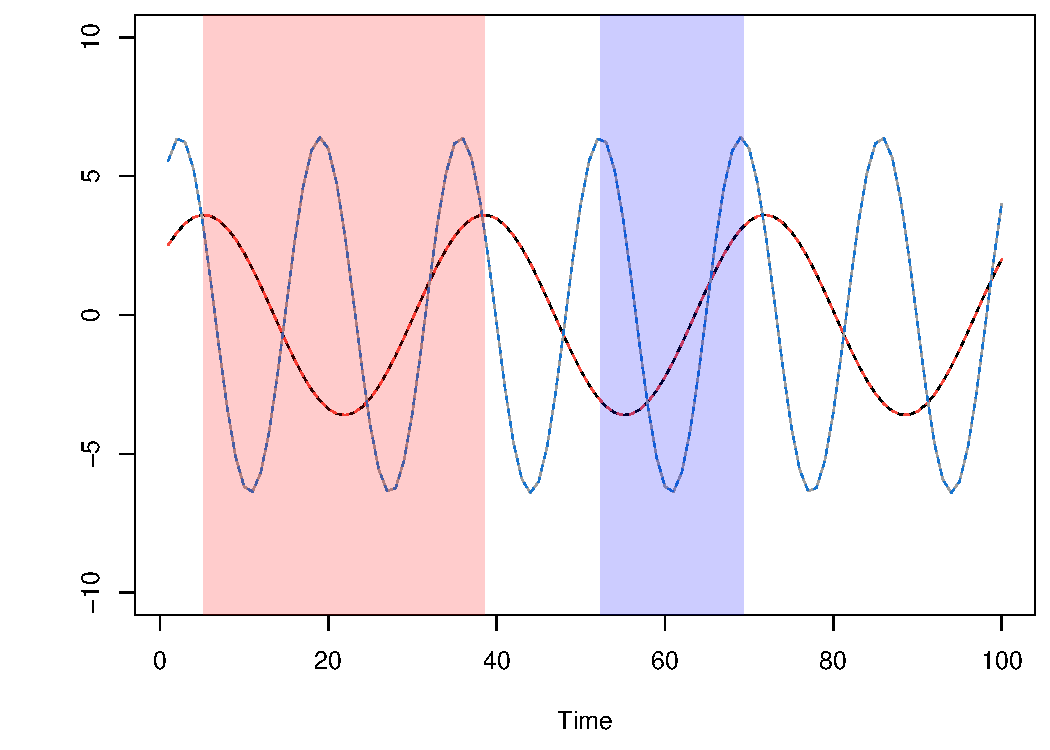
\includegraphics[width=0.85\textwidth]{fig/cos-process-1.pdf}
\caption{Two examples of cosine processes, the first (in red) having a frequency  
  $\omega = 3/100$ and amplitude \smash{$\sqrt{2^2 + 3^2} \approx 3.6$}, and the
  second (in blue) having a frequency $\omega = 6/100$ and amplitude
  \smash{$\sqrt{4^2 + 5^2} \approx 6.4$}.} 
\label{fig:cos_process}
\end{figure}

\item The quantity $A$ is called the \emph{amplitude} and $\phi$ the
  \emph{phase} of the process. The amplitude controls how high the peaks are, 
  and the phase determine where (along the cosine cycle) the process starts at
  the origin $t=0$   

\item We can introduce randomness into the process \eqref{eq:cos_process} by
  allowing $A$ and $\phi$ to be random

\item It will be useful to reparametrize. In general, recall the trigonometric
  identity (cosine compound angle formula):
  \begin{equation}
  \label{eq:compound_angle}
  \cos(a + b) = \cos(a) \cos(b) - \sin(a) \sin(b)
  \end{equation}
  Thus, starting with \eqref{eq:cos_process}, we can rewrite this as $x_t$ = $A
  \cos(\phi) \cos(2\pi\omega t) - A \sin(\phi) \sin(2\pi\omega t)$. Simply
  letting $U_1 = A \cos(\phi)$, $U_2 = -A \sin(\phi)$, we can therefore write   
  \begin{equation}
  \label{eq:cos_sin_process}
  x_t = U_1 \cos(2\pi\omega t) + U_2 \sin(2\pi\omega t)
  \end{equation}
  with $U_1, U_2$ our two random variables, determining the amplitude of the
  cosine and sine components separately

\item Note that another way of writing the relationship between $A,\phi$ and
  $U_1,U_2$ is (why?):
  \[
  A = \sqrt{U_1^2 + U_2^2}, \quad \phi = \tan^{-1}(-U_2/U_1)
  \]

  \item An interesting fact (that you can try to verify as a challenge): 
  \[
  U_1,U_2 \sim N(0,1), \text{ independently} \iff 
  A \sim \chi^2_2, \; \phi \sim \mathrm{Unif}(-\pi,\pi), \text{ independently} 
  \]
\end{itemize}

\subsection{Stationarity}

\begin{itemize}
\item If $U_1,U_2$ are uncorrelated, each with mean zero and variance
  $\sigma^2$, then the periodic process $x_t$, $t = 1,2,3,\dots$ defined in
  \eqref{eq:cos_sin_process} is stationary 

\item To check this: simply compute the mean function
  \[
  \mu_t = \E(x_t) = 0
  \]
  which is constant in time; and the autocovariance function 
  \begin{align*}
  \gamma(s,t) &= \Cov(x_s, x_t) \\
  &= \Cov\Big( U_1 \cos(2\pi\omega s) + U_2 \sin(2\pi\omega s), \, 
    U_1 \cos(2\pi\omega t) + U_2 \sin(2\pi\omega t) \Big) \\
  &= \Cov\Big( U_1 \cos(2\pi\omega s), \, U_1 \cos(2\pi\omega t) \Big) +
    \Cov\Big( U_2 \sin(2\pi\omega s), \, U_1 \cos(2\pi\omega t) \Big) \\
  &\qquad + \Cov\Big( U_1 \cos(2\pi\omega s), \, U_2 \sin(2\pi\omega t) \Big) +  
     \Cov\Big( U_2 \sin(2\pi\omega s), \, U_2 \sin(2\pi\omega t) \Big) \\
  &=\sigma^2 \cos(2\pi\omega s) \cos(2\pi\omega t) + 0 + 0 + \sigma^2
    \sin(2\pi\omega s) \sin(2\pi\omega t) \\
  &= \sigma^2 \cos(2\pi\omega (s-t))
  \end{align*}
  which only depends on the lag $s-t$ (where in the last line we used the
  identity \eqref{eq:compound_angle} once again)
\end{itemize}

\subsection{General mixtures}

\begin{itemize}
\item As a generalization of \eqref{eq:cos_sin_process}, we can also mix
  together a total of $p$ periodic processes, defining
  \begin{equation}
  \label{eq:cos_sin_process_p}
  x_t = \sum_{i=1}^p \Big( U_{j1} \cos(2\pi\omega_j t) + U_{j2}
  \sin(2\pi\omega_j t) \Big) 
  \end{equation}
  for $U_{j1}, U_{j2}$, $j = 1,\dots,p$ all uncorrelated random variables with
  mean zero, where $U_{j1}, U_{j2}$ have variance $\sigma^2_j$

\item As a generalization of the above calculation, you'll show on your homework
  that the process $x_t$, $t = 1,2,3,\dots$ defined in
  \eqref{eq:cos_sin_process_p} is stationary, with autocovariance function  
  \[
  \gamma(h) = \sum_{j=1}^p \sigma^2_j \cos(2\pi\omega_j h)
  \]

\item Figure \ref{fig:cos_mixture} displays a couple of mixture processes of the 
  form \eqref{eq:cos_sin_process_p} (with $p=2$ and $p=3$). Note the regular
  repeating nature of the mixture processes. One might wonder how we can
  decompose a such a mixture into its frequency components (periodic processes,
  each of the form \eqref{eq:cos_sin_process}). This is, in fact, one of the
  main objectives in spectral analysis

\begin{figure}[htb]
\centering
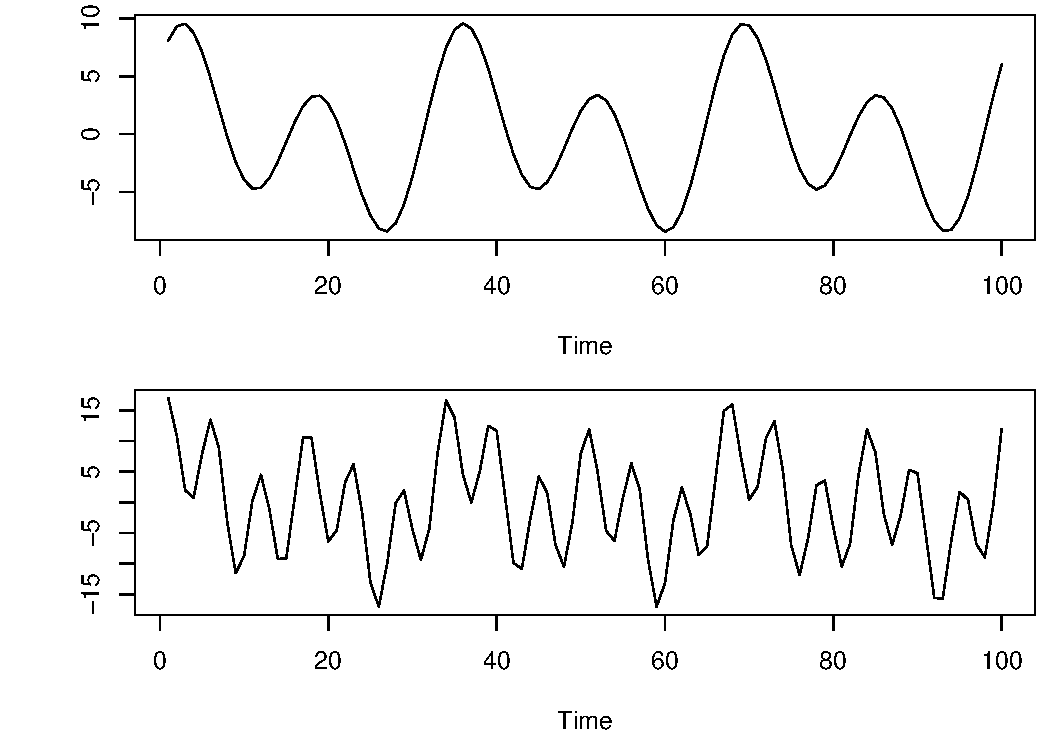
\includegraphics[width=0.875\textwidth]{fig/cos-mixture-1.pdf}
\caption{Mixture of periodic processes of different frequencies (and
  amplitudes).}  
\label{fig:cos_mixture}
\end{figure}

\item And the answer, as we'll see next, is given by something you're already
  quite familiar with ... regression! 
\end{itemize}

\section{Fourier decomposition}

\begin{itemize}
\item Given a time series $x_t$, $t = 1,\dots,n$, consider \emph{seeking} a
  decomposition like \eqref{eq:cos_sin_process_p}. We could do this by
  regressing this time series onto cosine and sine features of different
  frequencies,  
  \begin{align*}
  c_{tj} &= \cos(2\pi j/n \cdot t), \quad t = 1,\dots,n \\
  s_{tj} &= \sin(2\pi j/n \cdot t), \quad t = 1,\dots,n
  \end{align*}
  (which we call these ``basis functions'' in the context of this particular
  regression problem), and so the regression model is 
  \begin{equation}
  \label{eq:fourier_model}
  x_t \approx a_0 + \sum_{j=1}^p (a_j c_{tj} + b_j s_{tj}), \quad t = 1,\dots,n 
  \end{equation}
  Thus the regression coefficients $a_j,b_j$, $j = 1,\dots,p$ represent the 
  amplitudes 

\item How large should $p$ in the above regression model? That is, how many
  cosine and sine basis functions do we need? An amazing fact (at least, it will
  probably seem amazing if you've never seen Fourier decomposition before): 
  \emph{for any time series $x_t$, $t = 1,\dots,n$, we only need to set $p =
    (n-1)/2$, and then the representation in \eqref{eq:fourier_model} will be 
    exact!}  

\item That is, there are coefficients \smash{$\hat{a}_j, \hat{b}_j$}, $j =
  1,\dots,p$ that will give us an equalities in \eqref{eq:fourier_model}, for
  all $t$  

\item (This assumes that $n$ is odd; if $n$ is even, then we need to add an
  additional component $a_{n/2} \cos(\pi t) = a_{n/2} (-1)^t$, and the same
  claim holds: the representation is exact)  

\item To find the coefficients \smash{$\hat{a}_j, \hat{b}_j$}, $j = 1,\dots,p$,
  we can simply perform regresion (least squares). We let $x \in \R^n$ denote
  our time series represented as a vector, which serves as the response vector
  in our regression problem, and we assemble our cosine and sine basis functions
  into a feature matrix  
  \[
  Z = \begin{bmatrix}
  \frac{1}{\sqrt{2n}} & \cos(2\pi \frac{1}{n} \cdot 1) & \sin(2\pi \frac{1}{n}
  \cdot 1) & \cos(2\pi \frac{2}{n} \cdot 1) & \dots & \sin(2\pi \frac{n-1}{2n}
  \cdot 1) \\  
  \frac{1}{\sqrt{2n}}  & \cos(2\pi \frac{1}{n} \cdot 2) & \sin(2\pi \frac{1}{n}
  \cdot 2) & \cos(2\pi \frac{2}{n} \cdot 2) & \dots & \sin(2\pi \frac{n-1}{2n}
  \cdot 2) \\  
  \vdots & & & & & \\
  \frac{1}{\sqrt{2n}}  & \cos(2\pi \frac{1}{n} \cdot n) & \sin(2\pi \frac{1}{n}
  \cdot n) & \cos(2\pi \frac{2}{n} \cdot n) & \dots & \sin(2\pi \frac{n-1}{2n}
  \cdot n)  
  \end{bmatrix} \in \R^{n \times n}
  \]

\item We can then perform regression of $x$ on $Z$ in order to estimate the
  coefficients: 
  \[
  (Z^\T Z)^{-1} Z^\T x
  \]

\item However, something is very special about out matrix $Z$: it satisfies 
  $Z^\T Z = (n/2) \cdot I$, where $I$ the $n \times n$ identity matrix. In other
  words, \emph{its columns are uncorrelated, and have squared $\ell_2$ norm
    equal to $n/2$}. This is a very special property of the cosine and sine
  basis functions (and it is the foundation of the discrete Fourier transform,
  to be discussed shortly)
    
\item Thus, writing $z_j$, $j = 1,\dots,n$ as the columns of $Z$, we have
  \renewcommand{\arraystretch}{1.3} 
  \[
  (Z^\T Z)^{-1} Z^\T x = \begin{bmatrix} \frac{2}{n} z_1^\T x \\ \frac{2}{n}
    z_2^\T x \\ \vdots \\ \frac{2}{n} z_n^\T  x \end{bmatrix},
  \]
 \renewcommand{\arraystretch}{1} 
  so the multiple regression coefficients of $x$ on $Z$ are simply the marginal
  regression coefficients

\item In other words, the coefficients are simply \smash{$\hat{a}_0 =
    \bar{x}$}, and 
  \begin{equation}
  \label{eq:fourier_coef}
  \begin{aligned}
  \hat{a}_j &= \frac{2}{n} c_j^\T x = \frac{2}{n} \sum_{t=1}^n x_t \cos(2\pi j/n
  \cdot t) \\
  \hat{b}_j &= \frac{2}{n} s_j^\T x = \frac{2}{n} \sum_{t=1}^n x_t \sin(2\pi j/n
  \cdot t) 
  \end{aligned}
  \end{equation}

\item And to be perfectly clear, this gives us the exact decomposition 
  \begin{equation}
  \label{eq:fourier_decomp}
  x_t = \bar{x} + \sum_{j=1}^{(n-1)/2} \Big( \hat{a}_j \cos(2\pi j/n \cdot t) + 
  \hat{b}_j \sin(2\pi j/n \cdot t) \Big), \quad t = 1,\dots,n 
  \end{equation}
  The reason: because $Z$ is orthogonal, it has $n$ linearly independent
  columns in $n$ dimensions, so we can exactly represent any vector as a linear
  combination of its columns---which means that the fitted values from
  regressing $x$ on $Z$ will be exactly $x$  

\item (Side note on computation: at first glance, in order to compute each
  \smash{$\hat{a}_j$} or \smash{$\hat{b}_j$}, we require $O(n)$ operations, and 
  so computing all of them should take $O(n^2$) time ... but in fact the
  \emph{entire set of} coefficients \smash{$\hat{a}_j, \hat{b}_j$}, $j =
  1,\dots,(n-1)/2$ can be computed in $O(n \log{n})$ time using what is known as
  the fast Fourier transform, which we'll return to below)
\end{itemize}

\subsection{Periodogram}

\begin{itemize}
\item Given a series $x_t$, $t = 1,\dots,n$, we can define an object from the
  coefficients \eqref{eq:fourier_coef} in the decomposition
  \eqref{eq:fourier_decomp} that is called the \emph{periodogram}, denoted 
  $P_x$. This takes values at frequencies $j/n$, for $j = 1,\dots,(n-1)/2$, and
  is defined by    
  \begin{equation}
  \label{eq:periodogram}
  P_x(j/n) = \frac{n}{4} \big( \hat{a}_j^2 + \hat{b}_j^2 \big)
  \end{equation}
  (The scaling by $n/4$ is unimportant but will be helpful for mapping this onto
  the discrete Fourier transform, later)

\item Large values of the periodogram indicate which frequencies are predominant
  in the given series. This is illustrated in Figure \ref{fig:periodogram},
  which displays the periodogorams for the two series in Figure
  \ref{fig:cos_mixture} 

\item If we think back to the mixture process \eqref{eq:cos_sin_process_p} as a
  model for our data, then the periodogram gives us a breakdown of which
  frequencies are the largest \emph{sources of variance}: recall $\sigma_j^2 =
  \E(U_{j1}^2 + U_{j2}^2)/2$ is the variance at frequency $\omega_j$ 

\begin{figure}[htb]
\centering
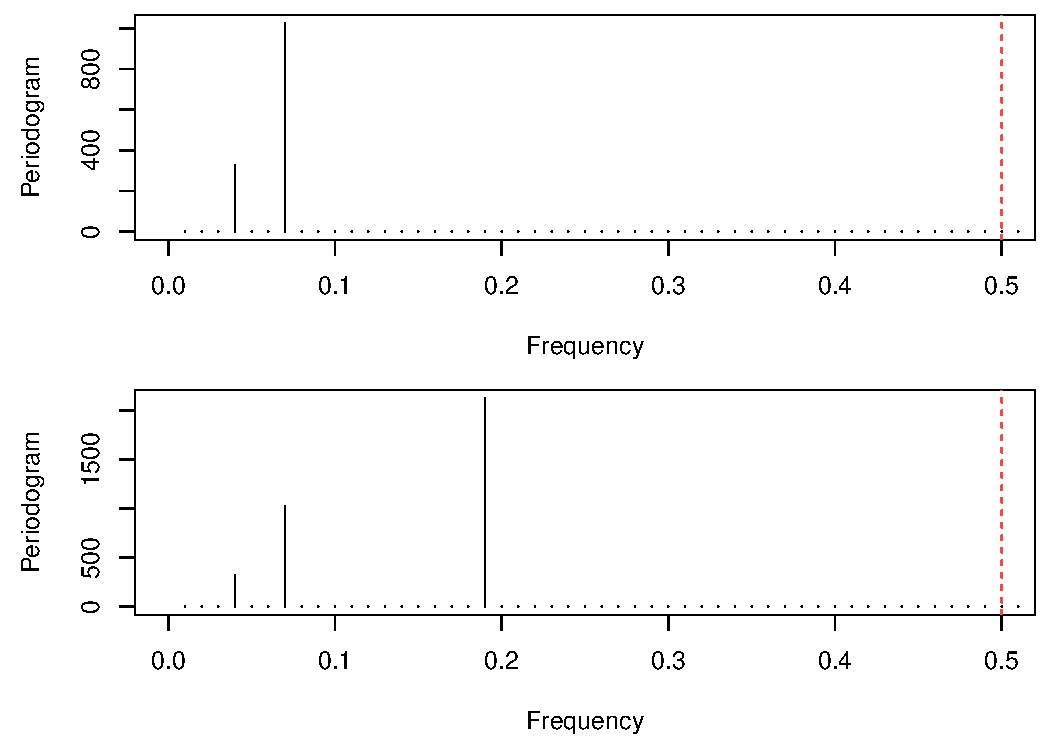
\includegraphics[width=0.875\textwidth]{fig/periodogram-1.pdf}
\caption{Periodograms for the mixture processes in Figure
  \ref{fig:cos_mixture}.} 
\label{fig:periodogram}
\end{figure}
\end{itemize}

\subsection{Discrete Fourier transform}

\begin{itemize}
\item The coefficients \eqref{eq:fourier_coef} used in the decomposition
  \eqref{eq:fourier_decomp} can be computed efficiently by recognizing their
  connection to what is called the \emph{discrete Fourier transform} (DFT) 

\item The DFT of a series $x_t$, $t = 1,\dots,n$, is denoted $d_x$ and defined
  as 
  \begin{equation}
  \label{eq:dft}
  d_x(j/n) = \frac{1}{\sqrt{n}} \sum_{t=1}^n x_t \exp(-2\pi i j/n \cdot t),
  \quad j = 0,1,\dots,n-1 
  \end{equation}
  where $i$ is the imaginary unit, which satisfies $i^2 = -1$. Thus the DFT is
  complex-valued  

\item Recalling Euler's formula, $e^{i\theta} = \cos(\theta) + i \sin(\theta)$, 
  we also have (using the fact that cosine is an even function and sine is odd): 
  \[
  d_x(j/n) = \frac{1}{\sqrt{n}} \sum_{t=1}^n x_t \cos(2\pi j/n \cdot t) - 
  \frac{i}{\sqrt{n}} \sum_{t=1}^n x_t \sin(2\pi j/n \cdot t), \quad j =
  0,1,\dots,n-1   
  \]

\item Thus, from the DFT, we can compute each cosine and sine coefficient in
  \eqref{eq:fourier_coef} by
  \[
  \hat{a}_j = \frac{2}{\sqrt{n}} \mathrm{Re}\{d_x(j/n)\} \quad \text{and} \quad 
  \hat{b}_j = -\frac{2}{\sqrt{n}} \mathrm{Im}\{d_x(j/n)\}
  \]
  where for a complex number $z = a+bi$, we use $\mathrm{Re}\{z\} = a$ and
  $\mathrm{Im}\{z\} = b$ to denote its real and imaginary parts

\item Note the following interesting connection to the periodogram. Since the
  the modulus of each entry of the DFT satisfies (by definition) $|d_x(j/n)|^2 = 
  \mathrm{Re}\{d_x(j/n)\}^2 + \mathrm{Im}\{d_x(j/n)\}^2$, the periodogram in
  \eqref{eq:periodogram} is 
  \begin{align*}
  P_x(j/n) &= \frac{n}{4} \big( \hat{a}_j^2 + \hat{b}_j^2 \big) \\
  &= \frac{n}{4} \bigg( \frac{4}{n} \mathrm{Re}\{d_x(j/n)\}^2 +
    \frac{4}{n} \mathrm{Im}\{d_x(j/n)\}^2 \bigg) \\
  &= |d_x(j/n)|^2
  \end{align*}
  That is, the periodogram is simply the squared modulus of the DFT 

\item Side note: the entire DFT $d_x$ can be computed rapidly using an algorithm
  called the fast Fourier transform (FFT), which takes $O(n\log{n})$ operations
  (most efficient in practice when $n$ is a highly composite integer, such as a
  power of 2). The modern generic FFT algorithm is credited to Cooley and Tukey
  in the 1960s, but similar ideas were arround much earlier   

\item Side side note: different software implementations scale the FFT/DFT 
  differently, so you have to be careful to consult the documentation. For
  example, the \verb|fft()| function in R computes it without the leading factor
  of $n^{-1/2}$, and with an additional factor of $\exp(2\pi i j/n)$ that can be
  ignored since we're only using it in our examples for its squared modulus, 
  i.e., the periodogram
\end{itemize}

\section{Spectral density}

\section{Linear filtering}

\section{Lagged regression}

\end{document}
